\documentclass{beamer}
\usepackage{beamerthemeshadow}
\usepackage[spanish]{babel}
\usepackage[utf8]{inputenc}
\usepackage[T1]{fontenc}
\usepackage{enumerate}
\usepackage{mathtools}
\usepackage{mathpazo}
\usepackage{amssymb}
\usepackage{stmaryrd}
\usepackage{lmodern}

%\setbeamertemplate{theorems}[ams style] % numbered
\theoremstyle{definition}
\makeatletter
\setbeamertemplate{theorem begin}
{%
  \inserttheoremheadfont \bfseries
  \inserttheoremname \inserttheoremnumber
  \ifx\inserttheoremaddition\@empty\else\ (\inserttheoremaddition)\fi%
  :
  \normalfont
}
\setbeamertemplate{theorem end}{%
  % empty
}
\makeatother

\newcommand{\until}{\mathrel{\mathbf{U}}}
\newcommand{\rel}{\mathrel{\mathbf{R}}}
\newcommand{\opnext}{\mathbf{X}}
\newcommand{\allp}{\mathbf{A}}
\newcommand{\existsp}{\mathbf{E}}
\newcommand{\squarep}{\mathbf{G}}
\newcommand{\lozp}{\mathbf{F}}
\newcommand{\formul}[3]{\llbracket #1, #2 \rrbracket_{#3}}
\newcommand{\dcorch}[1]{\llbracket #1 \rrbracket}
\newcommand{\ldcorch}[1]{\prescript{}{l}{\llbracket #1 \rrbracket}}
\newcommand{\eqdef}{:=}

\newtheorem{defin}{Definición}
\newtheorem{propo}[defin]{Proposición}
\newtheorem{teom}[defin]{Teorema}
\newtheorem{lema}[defin]{Lema}
\newtheorem{cor}{Corolario}[defin]
\newtheorem*{acl}{Aclaraciones}

\begin{document}
\title{Symbolic Model Checking Without BDDs}
\author{Gabriel Thibeault y Gonzalo Ciruelos}
\date{27 de noviembre de 2017}


%\frame{\titlepage}

\section{Introducción}
\frame{\frametitle{El trabajo}
\begin{center}
    Symbolic Model Checking withouth BDDs
\end{center}
    \vspace{2em}
Autores:
\begin{itemize}
    \item Armin Biere$^1$
    \item Alessandro Cimatti$^2$
    \item Edmund Clarke$^1$
    \item Yunshan Zhu$^1$
\end{itemize}
$^1$ Departamento de Computación de la Universidad de Carnegie Mellon

$^2$ Instituto de Investigación Científica y Tecnológica de Provo, Italia
}

\frame{\frametitle{Contexto}
El model checking es una técnica para verificar sistemas reactivos dado un sistema de transición que lo represente y una especificación (usualmente en lógicas temporales).
\bigskip

Symbolic model checking es una técnica que usa una representación canónica (mediante el uso de OBDDs) de los sistemas de transición y de las fórmulas a chequear.
\bigskip

Dicha representación maneja hasta el orden de $10^{20}$ estados, para sistemas más complejos, el cómputo se vuelve intratable.

}

\frame{\frametitle{Motivación}
Sin embargo, los OBDDs son muy sensibles al orden de las variables y además, en el peor caso su tamaño no es polinomial en la cantidad de variables.
\bigskip

En este trabajo presentan un una técnica basada en SAT para model checking simbólico. La idea es considerar contraejemplos de un cierto tamaño y generar una fórmula proposicional que sea satisfacible si y solo si existe tal contraejemplo.
\bigskip

La ventaja es que la reducción se puede hacer en tiempo polinomial y no requiere la construcción del
autómata completo.

El método propuesto es muy rápido , dada la naturaleza depth-first de SAT, y además encuentra contraejemplos de longitud mínima.
}

\section{Desarrollo}
\frame{\frametitle{Definiciones}
\begin{defin} 
    Una estructura de Kripke es una tupla $M = (S, I, T, \ell)$ con un conjunto finito de
    estados $S$, un conjunto de estados iniciales $I \subseteq S$, una relación de transición $T \subseteq S \times S$, y un etiquetado de estados $\ell : S \to \mathcal{P}(A)$ de proposiciones atómicas $A$.
\end{defin} 
\bigskip

\begin{acl}
\begin{itemize}
  \item Usamos una codificación binaria de las variables.
  \item $f_I(s) \iff s \in I$.
  \item $f_p(s) \iff p \in \ell(s)$.
  \item $(s, t) \in T \iff s \to t$.
  \item $\pi = (s_0, s_1, ...)$ definimos $\pi_i = s_i$ y $\pi^i = (s_i, s_{i+1}, ...)$.
\end{itemize}
\end{acl}
}

\frame{\frametitle{Definiciones...}
\begin{defin}[Semántica]
    Dada una estructura de Kripke $M$, un camino $\pi$ en $M$, $f$ una fórmula de LTL. Entonces $\pi \models f$ ($f$ es válido a lo largo de $\pi$) se define:

\begin{itemize}
  \item $\pi \models p \iff p\in \ell(\pi_0)$
  \item $\pi \models \neg p \iff p \not\in \ell(\pi_0)$
  \item $\pi \models f \land g \iff \pi \models f \text{ y } \pi \models g$
  \item $\pi \models f \lor g \iff \pi \models f \text{ o } \pi \models g$
  \item $\pi \models \squarep f \iff \forall i, \pi^i \models f$
  \item $\pi \models \lozp f \iff \exists i, \pi^i \models f$
  \item $\pi \models \opnext f \iff \pi^1 \models f$
  \item $\pi \models f \until g \iff \exists i , ( \pi^i \models g \text{ y } \forall j < i, \pi^j \models f)$
  \item $\pi \models f \rel g \iff \forall i ,   ( \pi^i \models g \text{ o } \exists j < i, \pi^j \models f)$
\end{itemize}
\end{defin}
}


\frame{\frametitle{Definiciones... (cont.)}
\begin{defin}[Validez]
    Una fórmula LTL $f$ es universalmente válida en una estructura de Kripke $M$ ($M \models \allp f$)$ \iff \pi \models f$ para todos los caminos $\pi$ en $M$ con $\pi_0 \in I$.
    Una fórmula LTL $f$ es existencialmente válida en una estructura de Kripke $M$ ($M \models \existsp f$)$ \iff \pi \models f$ para algún camino $\pi$ en $M$ con $\pi_0 \in I$.
\end{defin}

\bigskip
\begin{propo}
  $M \models \allp f   \iff   M \not\models \existsp \neg f$
\end{propo}

% Es claro que una fórmula LTL $f$ es universalmente válida en una estructura de Kripke si y solo si su negación no es existencialmente válida.

\bigskip
Reducimos la búsqueda de un contraejemplo de $\allp f$ a la búsqueda de una traza que satisfaga $\neg f$.

\bigskip
La idea básica del bounded model checking es considerar solo un prefijo finito de un camino que sea solución al problema de model checking existencial.
}

\frame{\frametitle{Loops}
Que consideremos sólo prefijos finitos no quiere decir que consideremos sólo caminos finitos.

\bigskip
Un prefijo finito puede representar un camino infinito si el prefijo contiene un loop.

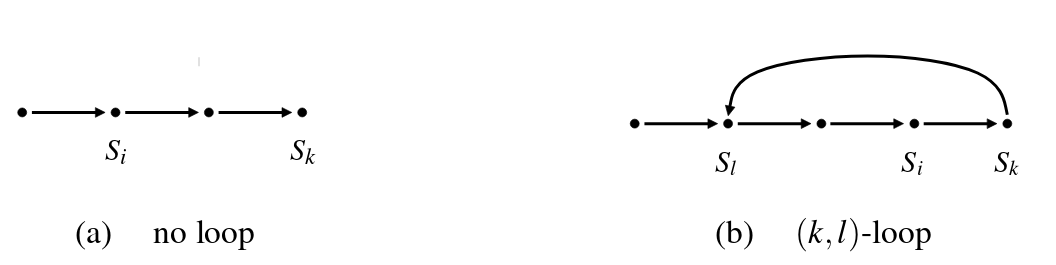
\includegraphics[width=10cm]{images/fig2.png}
}

\frame{\frametitle{Loops}
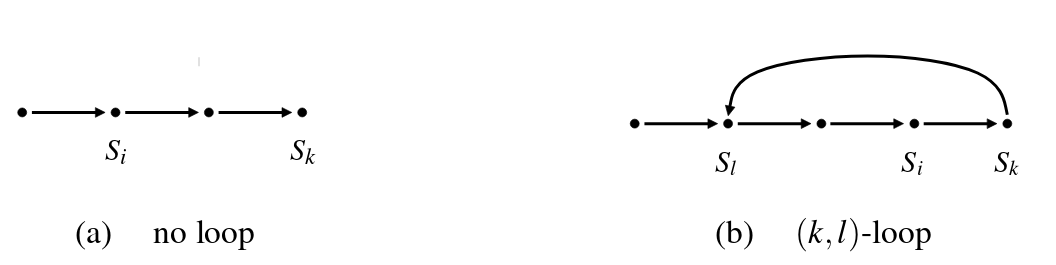
\includegraphics[width=10cm]{images/fig2.png}
\begin{defin}
    Para $l \leqslant k$ llamamos a un camino $\pi$ un $(k,l)$-loop si $\pi_k \to \pi_l$
y $\pi = u v^{\omega}$ con $u = (\pi_0, ..., \pi_{l - 1})$ y $v = (\pi_l, ..., \pi_k)$.
Llamamos a $\pi$ simplemente un $k$-loop si hay un $l \in \mathbb{N}$ tal que $l \leqslant k$ para el cual $\pi$
es un $(k, l)$-loop.
\end{defin}

\bigskip
\begin{defin}[Semántica acotada para trazas con loop]
Sea $k \in \mathbb{N}$, $\pi$ un $k$-loop y $f$ una fórmula LTL.
$\pi \models_k f \iff \pi \models f$.
\end{defin}
}

\frame{\frametitle{Loops}
\begin{defin}[Semántica acotada para trazas sin loops]
Sea $k \in \mathbb{N}$, $\pi$ una traza que no es un $k$-loop y $f$ una fórmula LTL.

$\pi \models_k f \iff \pi \models^0_k f$
\end{defin}

\begin{itemize}
  \item $\pi \models^i_k p \iff p\in \ell(\pi_i)$
  \item $\pi \models^i_k \neg p \iff p \not\in \ell(\pi_i)$
  \item $\pi \models^i_k f \land g \iff \pi \models^i_k f \text{ y } \pi \models^i_k g$
  \item $\pi \models^i_k f \lor g \iff \pi \models^i_k f \text{ o } \pi \models^i_k g$
  \item $\pi \models^i_k \squarep f \iff False$
  \item $\pi \models^i_k \lozp f \iff \exists i \leqslant j \leqslant k. \pi \models^j_k f$
  \item $\pi \models^i_k \opnext f \iff i < k \text{ y } \pi \models^{i+1}_k f$
  \item {\small $\pi \models^i_k f \until g \iff \exists j, i \leqslant j \leqslant k [ \pi \models^j_k g \text{ y } \forall n, i \leqslant n < j, \pi \models^n_k f]$}
  \item {\small $\pi \models^i_k f \rel g \iff \exists j, i \leqslant j \leqslant k [ \pi \models^j_k f \text{ y } \forall n, i \leqslant n < j, \pi \models^n_k g]$}
\end{itemize}
}


\frame{\frametitle{Todo anda}
\begin{lema}[Correctitud]
Sea $f$ una fórmula LTL, $k \in \mathbb{N}$ y $\pi$ un camino. 
$\pi \models_k f \implies \pi \models f$.
\end{lema}
\bigskip

\begin{lema}[Completitud para existenciales]
Sea $f$ una fórmula LTL, $M$ estructura de Kripke. 
$M \models \existsp f \implies \exists k \in \mathbb{N} /\ M \models_k \existsp f$.
\end{lema}
\bigskip

\begin{teom}[Correctitud y completitud para  existenciales]
Sea $f$ una fórmula LTL, $M$ estructura de Kripke. 
$M \models \existsp f \iff \exists k \in \mathbb{N} /\ M \models_k \existsp f$.
\end{teom}
}


\frame{\frametitle{Construyendo la fórmula}
Dada una estructura de Kripke $M$, una fórmula LTL $f$ y una cota $k$ construiremos la fórmula
proposicional $\formul{M}{f}{k}$. Las variables $s_0, ..., s_k$ de $\formul{M}{f}{k}$ representarán la secuencia de estados de un camino $\pi$. Cada $s_i$ es un vector de variables de estado.
\bigskip

La fórmula $\formul{M}{f}{k}$ representa esencialmente restricciones sobre $s_0, ..., s_k$ tal que $\formul{M}{f}{k}$ es satisfacible si y solo si $M \models_k \existsp f$.
\bigskip

El tamaño de $\formul{M}{f}{k}$ es polinomial en el tamaño de $f$, cuadrática en $k$ y lineal en el tamaño
de las fórmulas proposicionales para $T$, $I$ y $p \in A$.
}

\frame{\frametitle{Construyendo la fórmula (cont.)}
\begin{defin}[Desarrollando la condición de transición]
Dada una estructura de Kripke $M$ y una cota $k \in \mathbb{N}$:
\begin{center}
$\dcorch{M}_k \eqdef I(s_0) \land \bigwedge\limits_{i=0}^{k-1} T(s_i, s_{i+1})$
\end{center}
\end{defin}
}


\frame{\frametitle{Traduciendo las fórmulas LTL cuando no hay loop}
\begin{defin}[Traduciendo una fórmula LTL sin un loop]
Dada una fórmula LTL $f$ y $k, i \in \mathbb{N} /\ i \leqslant k$.
\end{defin}
\begin{itemize}
  \item $\dcorch{p}^i_k \eqdef p(s_i)$
  \item $\dcorch{\neg p}^i_k \eqdef \neg p(s_i)$
  \item $\dcorch{f \land g}^i_k \eqdef \dcorch{f}^i_k \land \dcorch{g}^i_k$
  \item $\dcorch{f \lor g}^i_k \eqdef \dcorch{f}^i_k \lor \dcorch{g}^i_k$
  \item $\dcorch{\squarep f}^i_k \eqdef False$
  \item $\dcorch{\lozp f}^i_k \eqdef \bigvee\limits_{j=i}^k \dcorch{f}_k^j$
  \item $\dcorch{\opnext f}^i_k \eqdef \text{ if } i < k \text{ then } \dcorch{f}_k^{i+1} \text{ else } False$
  \item {\small $\dcorch{f \until g}^i_k \eqdef \bigvee\limits_{j=i}^k \bigg(\dcorch{g}_k^j \land \bigwedge\limits_{n=i}^{j-1} \dcorch{f}_k^n \bigg)$}
  \item {\small $\dcorch{f \rel g}^i_k \eqdef \bigvee\limits_{j=i}^k \bigg(\dcorch{f}_k^j \land \bigwedge\limits_{n=i}^{j} \dcorch{g}_k^n \bigg)$}
\end{itemize}
}

\frame{\frametitle{Traduciendo las fórmulas LTL cuando hay loop}
\begin{defin}[Sucesor en un loop]
Sea $k, l, i, \in \mathbb{N}$, con $l, i \leqslant k$.
Definimos el sucesor $succ(i)$ de $i$ en un $(k,l)$-loop como $succ(i) = i + 1$ para $i < k$ y $succ(k) = l$.
\end{defin}

\begin{defin}
Dada una fórmula LTL $f$ y $k, l, i \in \mathbb{N} /\ l, i \leqslant k$.
\end{defin}

\begin{itemize}
  \item $\ldcorch{p}^i_k \eqdef p(s_i)$
  \item $\ldcorch{\neg p}^i_k \eqdef \neg p(s_i)$
  \item $\ldcorch{f \land g}^i_k \eqdef \ldcorch{f}^i_k \land \ldcorch{g}^i_k$
  \item $\ldcorch{f \lor g}^i_k \eqdef \ldcorch{f}^i_k \lor \ldcorch{g}^i_k$
  \item $\ldcorch{\squarep f}^i_k \eqdef \bigwedge\limits_{j=min(i,l)}^k \ldcorch{f}_k^j$
  \item $\ldcorch{\lozp f}^i_k \eqdef \bigvee\limits_{j=min(i,l)}^k \ldcorch{f}_k^j$
  \item $\ldcorch{\opnext f}^i_k \eqdef \ldcorch{f}^{succ(i)}_k$
\end{itemize}
}


\frame{\frametitle{Traduciendo las fórmulas LTL cuando hay loop (caso $f \until g$)}
\begin{center}
$\ldcorch{f \until g}^i_k \eqdef \bigvee\limits_{j=i}^k \bigg(\ldcorch{g}_k^j \land \bigwedge\limits_{n=i}^{j-1} \ldcorch{f}_k^n \bigg) \lor$
$\bigvee\limits_{j=l}^{i-1} \bigg(\ldcorch{g}_k^j \land \bigwedge\limits_{n=i}^{k} \ldcorch{f}_k^n
                                                 \land \bigwedge\limits_{n=l}^{j-1} \ldcorch{f}_k^n \bigg)$
\end{center}

% INSERTAR DIBUJO
}


\frame{\frametitle{Traduciendo las fórmulas LTL cuando hay loop (caso $f \rel g$)}
\begin{center}
$\ldcorch{f \rel g}^i_k \eqdef \bigwedge\limits_{j=min(i,l)}^k \ldcorch{g}_k^j \lor$

$\bigvee\limits_{j=i}^k \bigg(\ldcorch{f}_k^j \land \bigwedge\limits_{n=i}^{j} \ldcorch{g}_k^n \bigg) \lor$

$\bigvee\limits_{j=l}^{i-1} \bigg(\ldcorch{f}_k^j \land \bigwedge\limits_{n=i}^{k} \ldcorch{g}_k^n
                                                 \land \bigwedge\limits_{n=l}^{j} \ldcorch{g}_k^n \bigg)$
\end{center}
}

\frame{\frametitle{Terminando la construcción de la fórmula}
\begin{defin}[Condición de ciclo]
Dados $k,l \in \mathbb{N} /\ l \leqslant k$. $\prescript{}{l}{L}_k \eqdef T(s_k, s_l)$, $L_k \eqdef \bigvee\limits_{l=0}^k \prescript{}{l}{L}_k$.
\end{defin}
}

\frame{\frametitle{Terminando la construcción de la fórmula (cont.)}
\begin{defin}[Traducción general]
Sea $f$ una fórmula LTL, $M$ una estructura de Kripke y $k \in \mathbb{N}$.
\[
  \formul{M}{f}{k} \eqdef \dcorch{M}_k \land \bigg(
    \bigg( \neg L_k \land \dcorch{f}_k^0\bigg) \lor
    \bigvee\limits_{l=0}^k \bigg(\prescript{}{l}{L}_k \land \ldcorch{f}_k^0 \bigg) \bigg)
\]
\end{defin}
\bigskip

\begin{teom}[Correctitud del algoritmo]
$\formul{M}{f}{k}$ es satisfacible $ \iff M \models_k \existsp f$.
\end{teom}
\bigskip


\begin{cor}[Correctitud v2 del algoritmo]
$M \models \allp \neg f \iff \forall k \in \mathbb{N}, \formul{M}{f}{k}\text{ es insatisfacible}$.
\end{cor}
}

\frame{\frametitle{Cotas}
\begin{teom}
Dada una fórmula LTL $f$ y una estructura de Kripke $M$, sea $|M|$ la cantidad de
estados de $M$. 
$M \models \existsp f \iff \exists k \leqslant M \cdot 2^{|f|} /\ M \models_k \existsp f$.
\end{teom}
\bigskip

\begin{defin}[Diámetro del bucle]
Decimos que una estructura de Kripke $M$ tiene forma de lazo
si existen $u, v \in \mathbb{N}$ tal que para todo camino $p$ que empieza en un estado inicial, $p = u_p v_p^{\omega}$, donde $u_p$ y $v_p$ son secuencias de longitud finita de largo menor a $u$ y $v$ respectivamente.
En tal caso se define el diámetro del bucle de $M$ como $(u,v)$.
\end{defin}
\bigskip

\begin{teom}
Dada una fórmula LTL $f$ y una estructura de Kripke $M$ con forma de lazo, sea $(u,v)$ el
diámetro del bucle de $M$. 
$M \models \existsp f \iff \exists k \leqslant u + v /\ M \models_k \existsp f$.
\end{teom}
}

\section{Resultados}


\frame{\frametitle{Resultados}
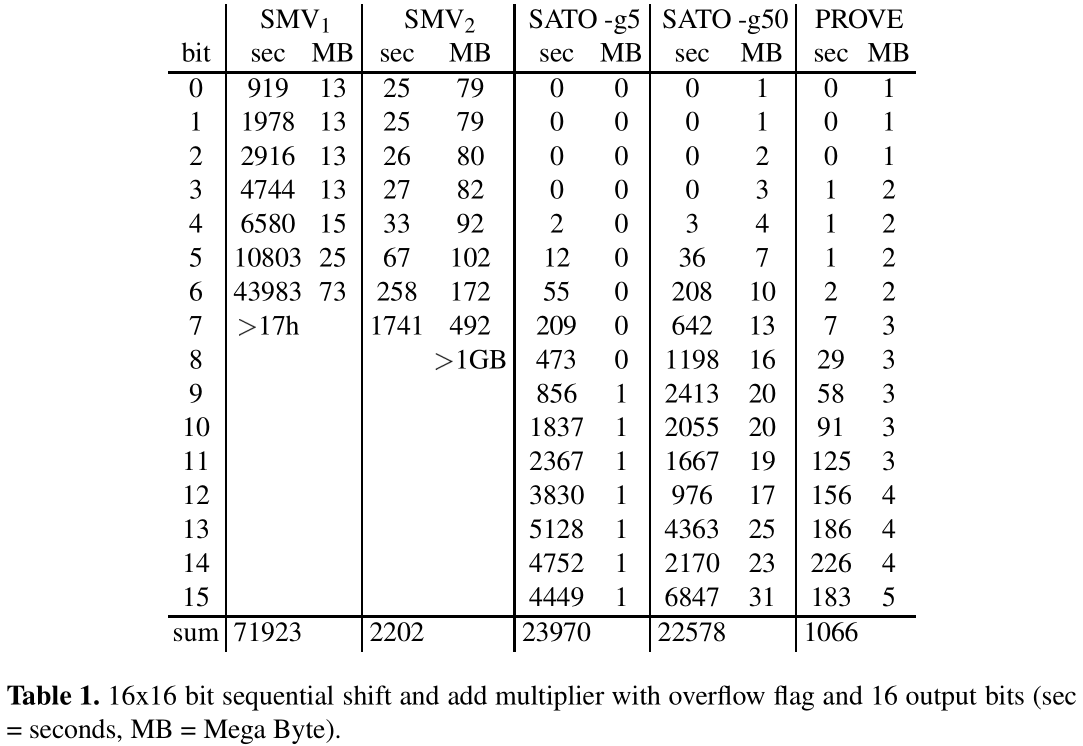
\includegraphics[width=10cm]{images/resultado1.png}
}

\frame{\frametitle{Resultados}
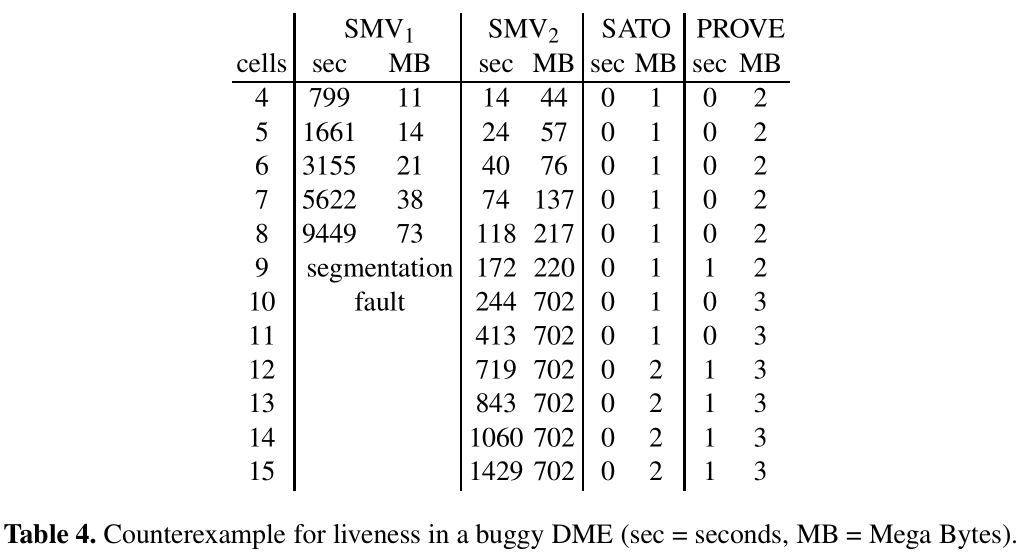
\includegraphics[width=10cm]{images/resultado2.png}
}


\frame{
\huge
\begin{center}
¿Preguntas?
\end{center}
}

\end{document}


